
\section{Case Study}
\label{sec:case-study}

\begin{figure}[t]
\centering
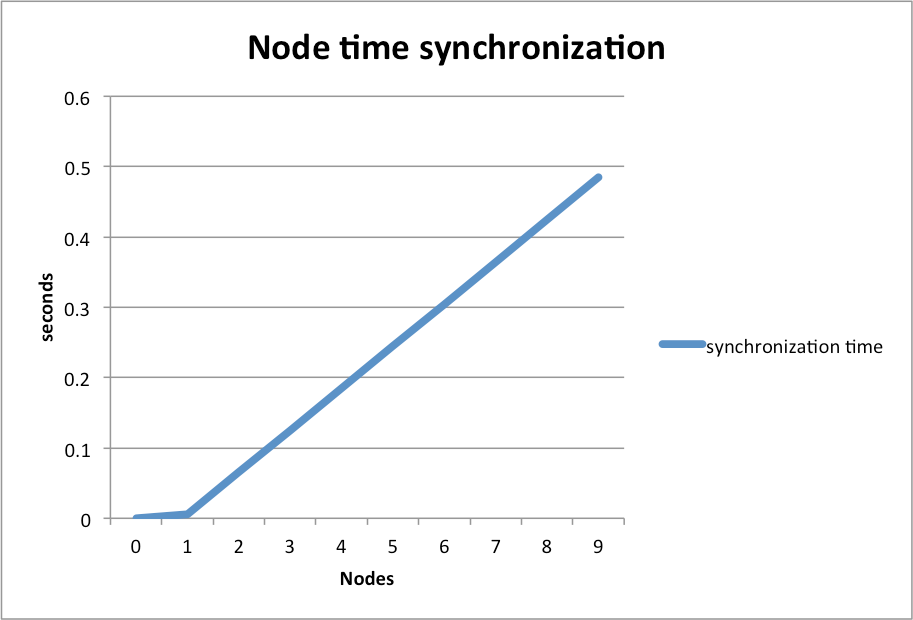
\includegraphics[width=1\columnwidth]{figures/timesynch}
\caption{Time Synchronization performance evaluation.}
\label{fig:timeCorrection}
\end{figure}


We considered a simple example to prove the effectiveness of the realized model.

Our setup included a set of 10 nodes with limited transmission power. Using the Wireless director, we configured each node to be able to communicate only with the previous and the successive node in the chain.
We analyzed how the time synchronization of the network.
\ben{To Be added later}.

%%% Local Variables: 
%%% mode: latex
%%% TeX-master: "ee219d"
%%% End: 
